\section{Beyond a Change of Basis: Polar Coordinates}

The preceding section changed the basis of the plane while keeping two fixed,
nonparallel vector directions. Polar coordinates make a more radical change:
they describe a point by distance and direction rather than by coefficients of
two fixed basis vectors.

\begin{corebox}[Linear and nonlinear coordinate changes]
A basis change keeps two fixed straight directions and produces a grid of
parallel lines. Polar coordinates use rays and concentric circles, and the
direction used to read the coordinates varies from point to point.
\end{corebox}

\subsection*{Two Different Questions About the Same Point}

\begin{corebox}[The polar questions]
Instead of asking for two signed projections, ask:
\begin{enumerate}
    \item How far is the point from the origin?
    \item In which direction must we move from the origin to reach it?
\end{enumerate}
\end{corebox}

\begin{definitionbox}
For a point different from the origin, its polar coordinates are
\[
\boxed{(r,\theta)},
\qquad
r>0,
\quad
0\leq\theta<2\pi,
\]
where $r$ is the Euclidean distance from the origin and $\theta$ is measured
counterclockwise from the positive $x$-axis.
\end{definitionbox}

\begin{definitionbox}
To make the representation unique in this course, the origin is represented only
by $(0,0)$. The allowed polar coordinate set is
\[
\boxed{
\mathcal P
=
\{(0,0)\}
\cup
\bigl((0,\infty)\times[0,2\pi)\bigr)
}.
\]
\end{definitionbox}

\begin{remarkbox}
In the usual nonunique convention, every pair $(0,\theta)$ represents the
origin. The restricted convention above is chosen only to give each point one
allowed coordinate pair.
\end{remarkbox}

\subsection*{Rectangular and Polar Grids}

\begin{center}
\begin{tikzpicture}[scale=0.78,>=stealth]
    \begin{scope}[xshift=0cm]
        \draw[gray!35,step=1] (-3.2,-3.2) grid (3.2,3.2);
        \draw[axis,->] (-3.4,0) -- (3.5,0) node[right] {$x$};
        \draw[axis,->] (0,-3.4) -- (0,3.5) node[above] {$y$};
        \coordinate (P1) at (2.4,1.8);
        \draw[helper,dashed] (P1) -- (2.4,0);
        \draw[helper,dashed] (P1) -- (0,1.8);
        \fill[geometricSubsetColor] (P1) circle (2.3pt) node[above right] {$P$};
        \node[align=center] at (0,-4.15)
            {Cartesian grid\\two families of parallel lines};
    \end{scope}

    \begin{scope}[xshift=9.2cm]
        \draw[axis,->] (-3.4,0) -- (3.5,0) node[right] {$x$};
        \draw[axis,->] (0,-3.4) -- (0,3.5) node[above] {$y$};
        \foreach \r in {1,2,3} {
            \draw[gray!45] (0,0) circle (\r);
        }
        \foreach \a in {0,30,...,330} {
            \draw[gray!45] (0,0) -- ({3.2*cos(\a)},{3.2*sin(\a)});
        }
        \coordinate (P2) at (2.4,1.8);
        \draw[very thick,->] (0,0) -- (P2) node[midway,above left] {$r$};
        \draw (0.8,0) arc[start angle=0,end angle=36.87,radius=0.8];
        \node at (1.05,0.34) {$\theta$};
        \fill[geometricSubsetColor] (P2) circle (2.3pt) node[above right] {$P$};
        \node[align=center] at (0,-4.15)
            {polar grid\\rays and concentric circles};
    \end{scope}
\end{tikzpicture}
\end{center}

\begin{interpretationbox}[Coordinate curves]
In Cartesian coordinates, $x=\text{constant}$ and $y=\text{constant}$ are
straight lines. In polar coordinates, $\theta=\text{constant}$ is a ray and
$r=\text{constant}$ is a circle. This visible difference shows that polar
coordinates are not merely a slanted basis.
\end{interpretationbox}

\subsection*{Converting Between the Descriptions}

\begin{derivationbox}[From polar to Cartesian]
The right triangle determined by a point with polar coordinates $(r,\theta)$
gives
\[
x=r\cos\theta,
\qquad
y=r\sin\theta.
\]
Hence
\[
\overrightarrow{OP}=r(\cos\theta,\sin\theta).
\]
\end{derivationbox}

\begin{theorembox}
The conversion from polar to Cartesian coordinates is
\[
\boxed{
x=r\cos\theta,
\qquad
y=r\sin\theta
}.
\]
\end{theorembox}

\begin{derivationbox}[From Cartesian to polar]
For $(x,y)\neq(0,0)$, the Euclidean distance formula gives
\[
r=\sqrt{x^2+y^2}.
\]
The direction is the unique $\theta\in[0,2\pi)$ satisfying
\[
\cos\theta=\frac{x}{r},
\qquad
\sin\theta=\frac{y}{r}.
\]
\end{derivationbox}

\begin{theorembox}
For $(x,y)\neq(0,0)$,
\[
\boxed{r=\sqrt{x^2+y^2}},
\]
and $\theta$ is determined by
\[
\boxed{
\cos\theta=\frac{x}{r},
\qquad
\sin\theta=\frac{y}{r}
}.
\]
\end{theorembox}

\begin{remarkbox}
The expression $\arctan(y/x)$ is insufficient because it loses quadrant
information and is undefined when $x=0$. In computation, the two-argument
function $\operatorname{atan2}(y,x)$ is used, with a negative output shifted by
$2\pi$ when the chosen range is $[0,2\pi)$.
\end{remarkbox}

\begin{examplebox}
For
\[
(r,\theta)=\left(2,\frac{\pi}{3}\right),
\]
we obtain
\[
x=2\cos\frac{\pi}{3}=1,
\qquad
y=2\sin\frac{\pi}{3}=\sqrt3.
\]
Thus the same point is written as $P=(1,\sqrt3)$ in Cartesian coordinates and as
$P=(2,\pi/3)$ in polar coordinates.
\end{examplebox}

\subsection*{Why the Transformation Is Nonlinear}

\begin{examplebox}
The polar pairs
\[
(1,0)
\qquad\text{and}\qquad
\left(1,\frac{\pi}{2}\right)
\]
represent Cartesian vectors $(1,0)$ and $(0,1)$. Their sum is $(1,1)$, whose
polar coordinates are
\[
\left(\sqrt2,\frac{\pi}{4}\right),
\]
not $(2,\pi/2)$. Polar coordinate pairs therefore cannot be added componentwise
to add vectors.
\end{examplebox}

\begin{interpretationbox}[What nonlinearity means here]
The formulas
\[
x=r\cos\theta,
\qquad
y=r\sin\theta
\]
contain trigonometric functions. The direction $(\cos\theta,\sin\theta)$ changes
with $\theta$, so $r$ and $\theta$ are not coefficients of two fixed basis
vectors.
\end{interpretationbox}

\subsection*{A Circle Becomes Simple}

Let
\[
C_R=\{(x,y)\in\mathbb R^2:x^2+y^2=R^2\},
\qquad R>0.
\]

\begin{derivationbox}[Rewriting the circle]
Substitute
\[
x=r\cos\theta,
\qquad
y=r\sin\theta.
\]
Then
\[
r^2\cos^2\theta+r^2\sin^2\theta=R^2.
\]
Using $\cos^2\theta+\sin^2\theta=1$ gives
\[
r^2=R^2.
\]
Since $r\geq0$ and $R>0$, this reduces to $r=R$.
\end{derivationbox}

\begin{theorembox}
The Cartesian equation
\[
x^2+y^2=R^2
\]
and the polar equation
\[
\boxed{r=R}
\]
describe the same circle.
\end{theorembox}

\begin{interpretationbox}[Choose coordinates adapted to the geometry]
Polar coordinates are efficient when distance from the origin is the dominant
feature. The geometric set does not change; only its coordinate language becomes
simpler.
\end{interpretationbox}

\begin{center}
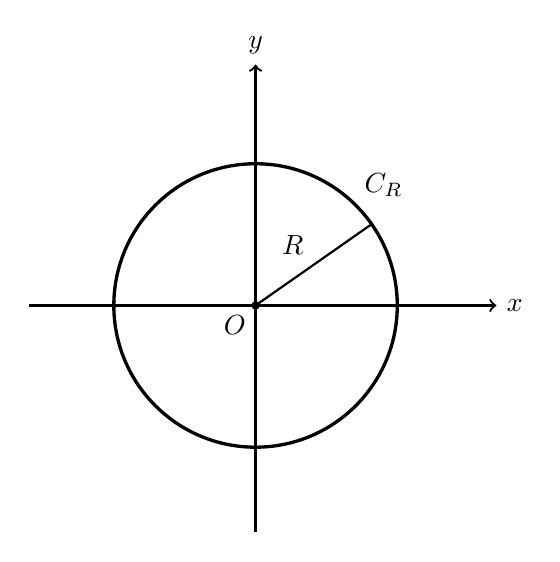
\begin{tikzpicture}[scale=0.9]
    \draw[->,thick] (-3.2,0) -- (3.4,0) node[right] {$x$};
    \draw[->,thick] (0,-3.2) -- (0,3.4) node[above] {$y$};
    \draw[very thick] (0,0) circle (2);
    \draw[thick] (0,0) -- ({2*cos(35)},{2*sin(35)})
        node[midway,above left] {$R$};
    \fill (0,0) circle (1.7pt) node[below left] {$O$};
    \node[above right] at (1.4,1.4) {$C_R$};
\end{tikzpicture}
\end{center}

\begin{summarybox}[First nonlinear coordinate system]
A basis uses fixed directions and leads to linear coordinate changes. Polar
coordinates use a distance and an angle:
\[
(r,\theta)\longleftrightarrow(r\cos\theta,r\sin\theta).
\]
Their coordinate curves are circles and rays, and vector addition is not
performed by adding polar coordinate pairs.
\end{summarybox}
